\documentclass[twoside,11pt,a4paper]{article}

\usepackage[utf8]{inputenc}
\usepackage[english]{babel}
\usepackage[T1]{fontenc}
\usepackage{graphicx}
\usepackage{subcaption}
\usepackage{amsmath}
\usepackage[subnum]{cases}
\usepackage{array}
\graphicspath{{pictures/}}
\usepackage{float}
\usepackage[pass]{geometry}	\usepackage{charter}
\usepackage{fancyhdr}
\usepackage{multirow}
\usepackage{charter}
\usepackage{enumitem}
\usepackage{textcomp}
\usepackage{gensymb}
\usepackage{breqn}
\usepackage{verbatim}
\usepackage{pdfpages}
%For bibliography
\usepackage[numbers]{natbib}
\usepackage{notoccite}
\usepackage{hyperref}

\newgeometry{margin=3cm}
\pagestyle{fancy}
\setlength{\headheight}{20pt}
\fancyhead[L]{\textsc{Master thesis}}
\renewcommand{\footrulewidth}{1pt} %forcer l'affichage de la ligne horizontale pour le pied de page%
\fancyfoot[R]{Page \thepage}
\fancyfoot[C]{}
\fancyfoot[L]{\textsc{Measurements of liners acoustic properties}}

\begin{document}

%-------------------------------------------------------------------------
%first page
\begin{titlepage}
    \begin{sffamily}
    \begin{center}
    \includegraphics[scale=0.7]{logokth.png}\\
    	\vspace{1cm}
    \LARGE{\textbf{INSA de Lyon \& Kungliga Tekniska högskolan}}\\
    \LARGE{\textbf{Master of science in acoustics}}
    	\vspace{1cm}
	\noindent\rule{15cm}{1pt}
		\vspace{1em}
		\Huge{\textbf{Master thesis - Projet de fin d'étude}}
		\vspace{1em}
		\Huge{\textbf{Measurements of liners acoustic properties}}	
	\noindent\rule{15cm}{1pt}
	\vspace{2cm}
    \end{center}        
    \begin{minipage}{0.5\textwidth}
      \begin{flushleft} \LARGE
        Francois \textsc{DAYET}\\
        June 2017
      \end{flushleft}
    \end{minipage}
    \begin{minipage}{0.45\textwidth}
      \begin{flushright} \large
        \emph{KTH responsible:}\\  
        \emph Hans \textsc{Bodén} \\  
        \emph{INSA responsible:} \\
        \emph Etienne \textsc{Parizet}
      \end{flushright}
    \end{minipage}
    \end{sffamily}
\end{titlepage} 
%-------------------------------------------------------------------------
%Acknowledgements
\pagestyle{empty}
\setlength{\parskip}{5pt}
\section*{Acknowledgements}
\setlength{\parindent}{20pt}
I'm grateful for the Marcus Wallenberg Laboratory for Sound and Vibration. It was a pleasure to work in this laboratory and use their facilities. It was for me a great opportunity to work in this acoustic environment.

I also want to show my gratitude to Luck Peerlings who helped me a lot. Thank you for your time and you very clear explanations. 

I want to specially thank my supervisor Hans Bodén. The subject he proposed was very interesting and stimulating. I learn a lot of acoustic knowledge thanks to him. He gave me the opportunity to do high valued measurements with a rare setup.

I thank my co-workers and all the people with I spent a great time. 

\clearpage 

%-------------------------------------------------------------------------
%Contents
\pagestyle{fancy}
\setcounter{page}{1}
\tableofcontents
\clearpage

%-------------------------------------------------------------------------
%Sections
\setlength{\parskip}{0pt}
\setlength\parindent{0pt}
\section{Introduction}
The noise pollution is one of the main issue of the XXI\textsuperscript{st} century. It causes usual annoyances but it also threat health. The European Union highlights the risks of noise pollution \cite{Noise_in_Europe}. The transports cause the highest noise pollution.  A considerable effort has be made to reduce the emissions and continue to be made.\\ 
In the aircraft field, the noise has to be reduced inside the structure in order to keep a relative comfort for the passengers and also outside in the case because aircraft fly over habitations. The main source of noise in the aircraft is the engines.\\
The emission of noise in an engine is complex and due to different phenomenon. Nowadays, the usual engines type is by-pass turbofan engine. At the input of the duct, there is the admission of low pressure air. A fan pushes the air into the higher levels, the interaction between this fan and the stator is one of the principal source of noise. Thus, a high air ratio pass trough the by-pass duct. The second path is the principal duct. The combustion is also a high source of emission. The air is ejection is called a jet flow. The interaction between the ejected air flows with different velocities is a source of noise. The following figure shows the different sources of noise in a by-pass turbofan engine.
\begin{figure}[H] \centering
    \includegraphics[scale=0.5]{Sources_in_engines}
    \caption{Different acoustic sources in engines \cite{Zhou_thesis}}
\end{figure}
To reduce the noise transmission, a liner acoustic is added in the engines walls. It is a perforated panel which contained a honeycomb structure. The small cavities can be compared to small Helmholtz resonators. The air in the orifices plays the role of mass and the cavity formed by the honeycomb structures acts as a spring.
\begin{figure}[H] \centering
\label{fig:Sources_in_engines2}
    \includegraphics[scale=0.4]{typical_perforate_liner}
    \caption{Typical perforate liner \cite{The_jet_engine}}
\end{figure}
Aircraft suppliers need to well understand how work these liners to optimize the geometry or to add some porous material inside the honeycomb structures. However the problem is very difficult. Indeed the size of the acoustic waves in the engines are larger than the size of the hole ($\sim$ 0.5mm). That's why it's very difficult to implement a finite-elements method. Some models are to be found to reduce this difficulty. The usual solution is to used the acoustic impedance of the liner:
\begin{itemize}
    \item First, the wall impedance is find with the acoustic theory applied to small cavities.
    \item The impedance of the liner is used in a macro model.
\end{itemize}
This master thesis is part of the IMAGE project (Innovative Methodologies and technologies for reducing Aircraft noise Generation and Emission) which is in collaboration with European and Chinese laboratories.
\clearpage 
\section{Theorical acoustic}\label{sec:section2}
%------------------------------------------------------------------------------------------------------------
%------------------------------------------------------------------------------------------------------------
%------------------------------------------------------------------------------------------------------------
%------------------------------------------------------------------------------------------------------------
\subsection{Acoustic in duct}
The acoustic in ducts is well-known and the main aspects were find by Helmholtz. A good overview can be found in this book \cite{Luck_thesis}.
We consider an infinite duct with x axis and a given section.

Acoustics is governed by few equations:
\begin{itemize}
    \item Mass continuity: 
        \begin{equation} 
        \frac{\partial \rho}{\partial t}+\mathrm{div}\rho v =0
        \end{equation}
    With $\rho$ the density, $v$ the velocity.
    \item Momentum continuity (given by the Navier-Stockes equation):
        \begin{equation} 
        \rho\frac{dv}{dt}=-\mathrm{grad} \rho+\mathrm{div} \tau+g
        \end{equation}
    \item energy continuity
\end{itemize}
However, these equations are too complex to be used analytically. Some assumptions are made:
\begin{itemize}
    \item Non-viscous fluid
    \item No thermal conductivity
    \item Entropy conservation
    \item Uniform mean flow
    \item Time dependence of $exp(iwt)$. The section is constant across the x axis. Thus $p\propto exp(iwt_\pm ikx)$
\end{itemize}
With the mass continuity and the momentum continuity, the convective Helmholtz equation can be found: 
    \begin{equation} 
    \Delta p +\Big[(w-ku_0)^2-k^2c_0^2\Big]p=0
    \end{equation}
With $\Delta$ the laplace operator and $c$ the speed velocity.\\
The solutions of this equations is a sum of different functions called modes: 
\begin{equation} 
    p(x,y,z,\omega)=\sum_{l=0}^\infty p_l^+ \Psi_l(y,z)e^{-ik_{x,l}(M,\omega)x}+p_l^- \Psi_l(y,z)e^{-ik_{x,l}(-M,\omega)x}
    \label{Convective_Helmholtz_Equation}
\end{equation}
With $M$ the mach number $M={v}/{c}$. The $l$ modes are sorted by frequency. Each mode has an acoustic shape in the section $(y,z)$. The mode can propagate in two different directions, in the positive or the negative direction.
The usual problem in acoustic is the significant number of modes which are not negligible. In the duct, only few modes propagate unattenuated. Indeed, over a certain cut-off frequency $Re(k_{x,l})$ is negative, these modes are attenuated very fast. This cut-off frequency depends of the geometry and the mach number. For usual duct, just one mode propagates energy, the plane wave mode.
%------------------------------------------------------------------------------------------------------------
\subsubsection{Rectangular duct} \label{sec:RectDuct}
To solve Eq.\eqref{Convective_Helmholtz_Equation}, the separation of variables method is used. The mode shapes are independent between the direction y and z (called $m$ modes for y direction and $n$ for z). For rigid wall boundary conditions:
\begin{equation} 
    \Psi_{m,n}(y,z)=\Psi_{m}(y)\Psi_{n}(z)=\cos(\frac{m\pi y}{2b})\cos(\frac{n\pi z}{2h})
\end{equation}
With $b$ and $h$ the width and the height.
The axial wave number $k_{x,(m,n)}$ is solution of dispersion equation: 
\begin{equation} 
    k_{x,(m,n)}=k_0\frac{M\pm\sqrt{1-(1-M^2)\Big[(\frac{m\pi}{2ka})^2+(\frac{n\pi}{2kh})^2\Big]}}{1-M^2}
\end{equation}
Mode will propagate if:
\begin{equation} 
    k\geq\sqrt{(1-M^2)\Big[(\frac{m\pi}{2a})^2+(\frac{n\pi}{2h})^2\Big]}
\end{equation}
The transverses waves numbers respect: 
\begin{equation} 
    k_{y,(m)}=\frac{m\pi}{2a} \ \text{and} \ k_{z,(n)}=\frac{n\pi}{2h}
\end{equation}
\begin{figure}[H] \centering
    \begin{subfigure}{.5\textwidth}\centering
     
\includegraphics[width=.8\linewidth]{modeR00}
     \caption{(0,0) plane wave mode}
    \end{subfigure}%
    \begin{subfigure}{.5\textwidth}\centering
     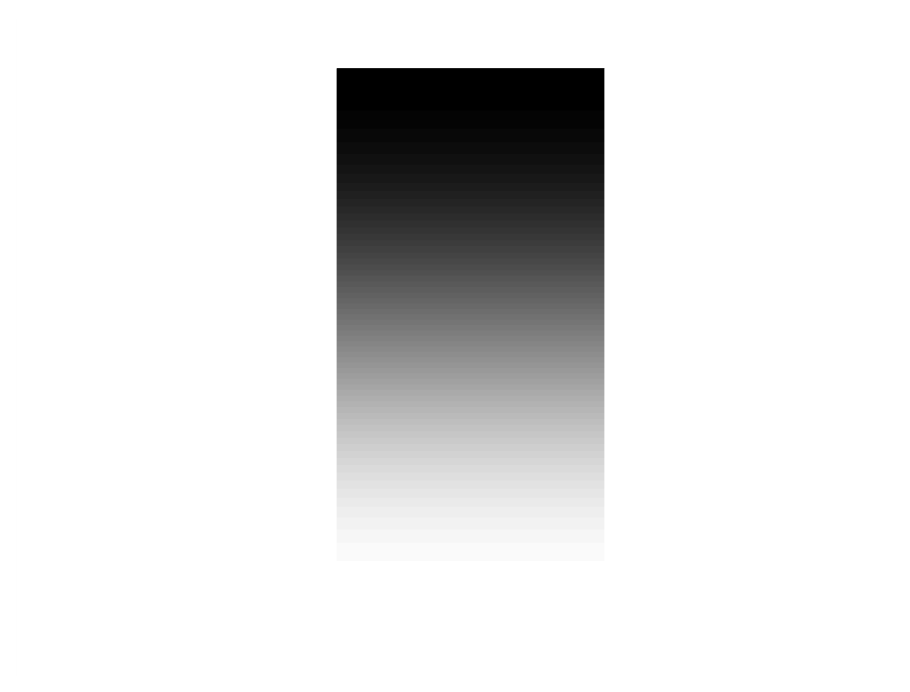
\includegraphics[width=.8\linewidth]{modeR01}
     \caption{(0,1)}
    \end{subfigure}\\
    \begin{subfigure}{.5\textwidth}\centering
     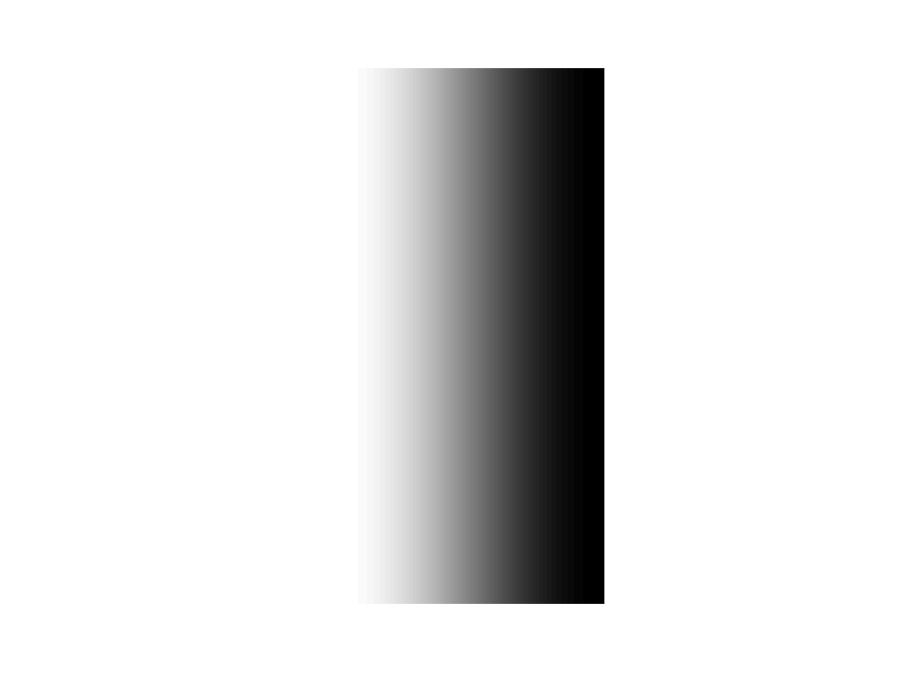
\includegraphics[width=.8\linewidth]{modeR10}
     \caption{(1,0)}
    \end{subfigure}%
    \begin{subfigure}{.5\textwidth}\centering
     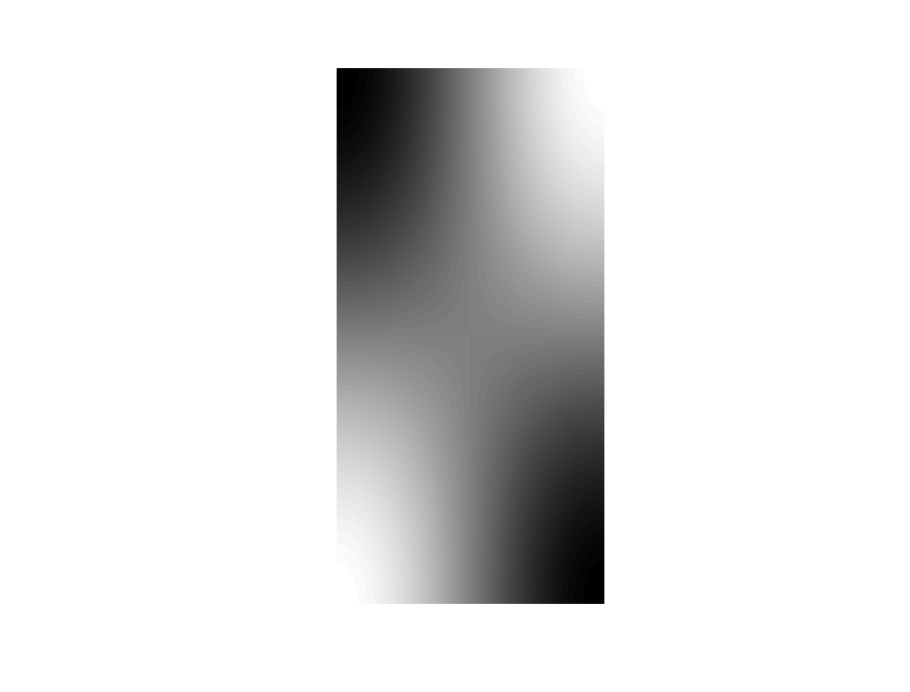
\includegraphics[width=.8\linewidth]{modeR11}
     \caption{(1,1)}
    \end{subfigure}
    \caption{Mode shape (m,n) in a rectangular duct}
\end{figure}
%------------------------------------------------------------------------------------------------------------
\subsubsection{Circular duct}
The radius is called R ($0<r<R$).
For circular duct, there are two kinds of modes: \textbf{circumferential and radial modes (called respectively $m$ and $n$)}. The mode shape is not independent between the radial and circumferential direction. 
\begin{equation} 
    \Psi_{m,n}(r,\theta)=J_m(k_{r,(m,n)} r)e^{jm\theta}
\end{equation}
Where $k_{r,(m,n)}=\frac{j_{mn}}{R}$. $J_m$ is the Bessel function and $j_{mn}$ is the n-th zero of $J_m^'$:
\begin{equation} 
    J_m^'(j_{mn})=0
\end{equation}
The axial wave number $k_{x,(m,n)}$ respect the dispersion equation: 
\begin{equation} 
    k_{x,(m,n)}=k_0\frac{M\pm\sqrt{1-(1-M^2)(\frac{j_{mn}}{kR})^2}}{1-M^2}
\end{equation}
Mode will propagate if:
\begin{equation} 
    kR\geq j_{mn}\sqrt{1-M^2}
\end{equation}
The radial wave number is: 
\begin{equation} 
    k_{r,(m,n)}=\frac{j_{mn}}{R}
\end{equation}
\begin{figure}[H] \centering
    \begin{subfigure}{.5\textwidth}\centering
     
\includegraphics[width=.8\linewidth]{modeC00}
     \caption{(0,0) plane wave mode}
    \end{subfigure}%
    \begin{subfigure}{.5\textwidth}\centering
     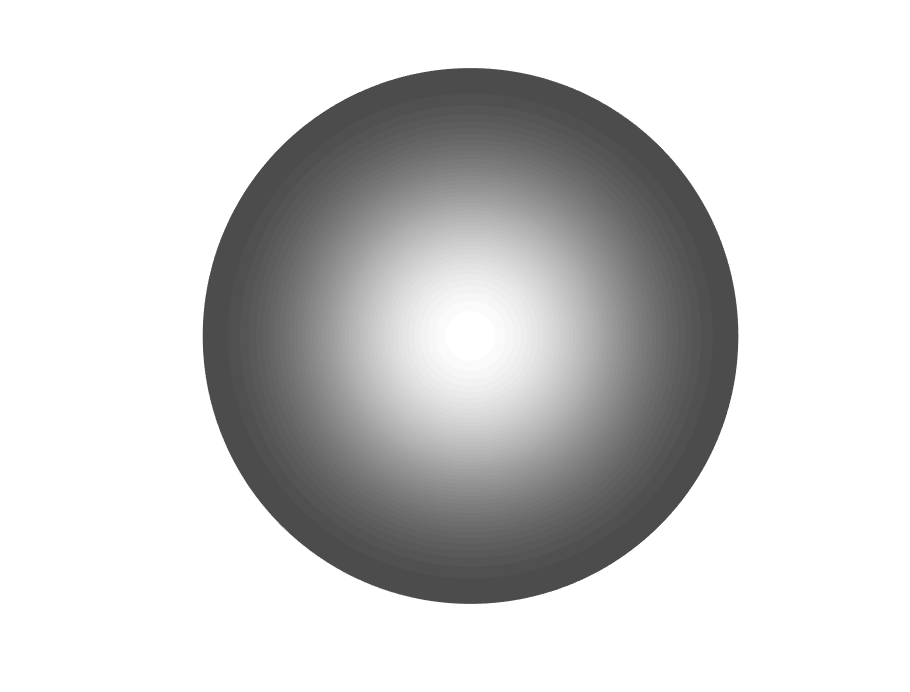
\includegraphics[width=.8\linewidth]{modeC01}
     \caption{(0,1)}
    \end{subfigure}\\
    \begin{subfigure}{.5\textwidth}\centering
     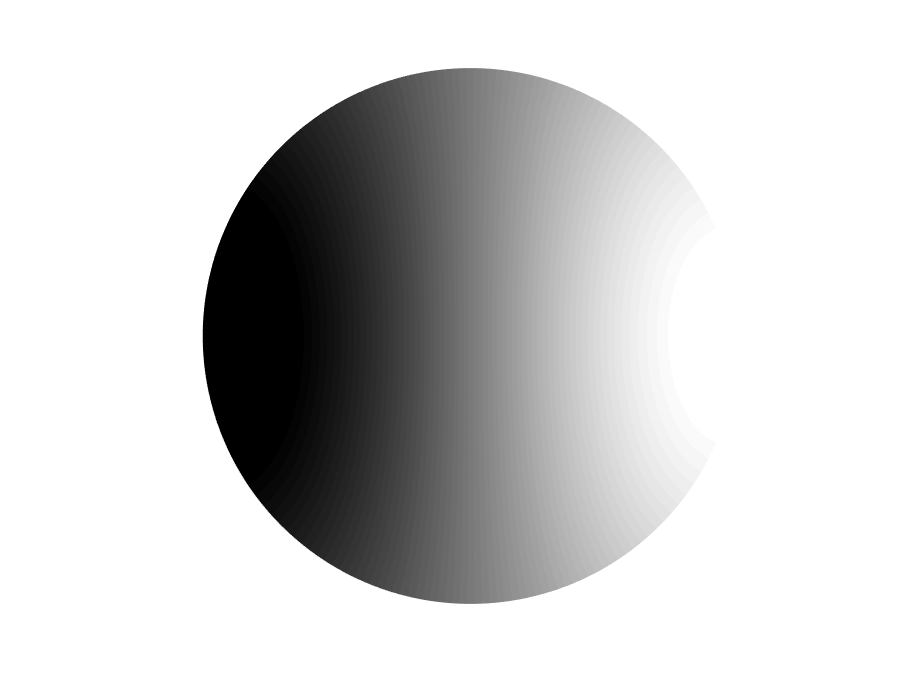
\includegraphics[width=.8\linewidth]{modeC10}
     \caption{(1,0)}
    \end{subfigure}%
    \begin{subfigure}{.5\textwidth}\centering
     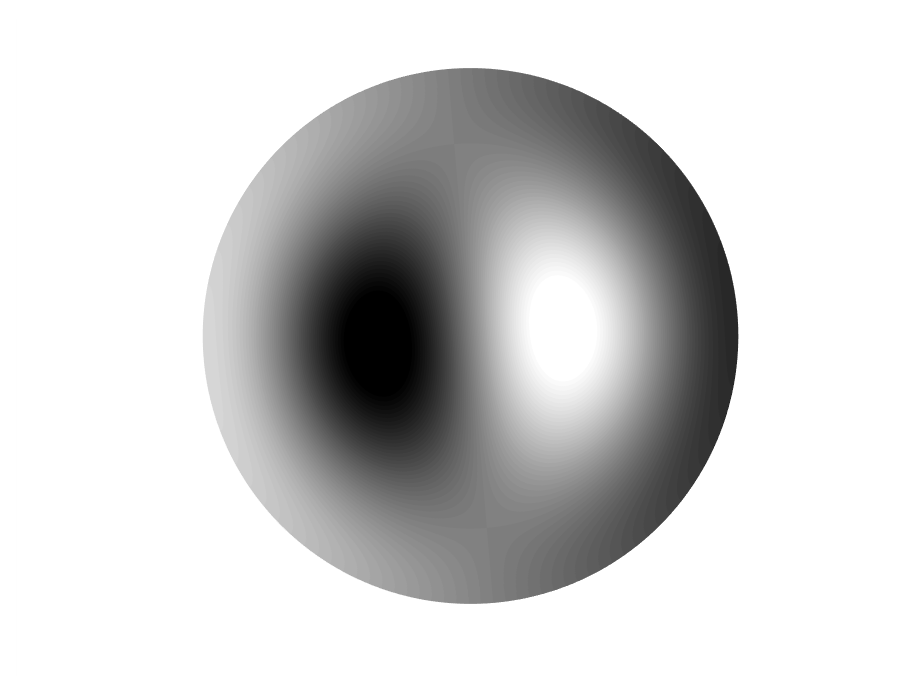
\includegraphics[width=.8\linewidth]{modeC11}
     \caption{(1,1)}
    \end{subfigure}
    \caption{Mode shape in a circular duct}
\end{figure}
%------------------------------------------------------------------------------------------------------------
\subsubsection{Wall attenuation}
\textbf{Model of attenuation}\\
The viscosity is not negligible at the interface wall/flow. A model of attenuation given by Pierce \cite{Pierce} is:
\begin{equation} 
    k=\frac{\omega}{c}+(1+i)\frac{1}{2\sqrt{2}}\sqrt{\frac{\omega\mu}{\rho c^2}}\Bigg[1+\frac{\gamma -1}{\sqrt{Pr}}\Bigg]\frac{L_p}{A}
\end{equation}
$Pr$ is the Prandtl number, $\rho$ the density, $L_p$ the perimeter and $A$ the area. An easy way to use attenuation is to replace $k_0=k$\smallbreak
\noindent\textbf{Boundary condition: Ingard-Myers}\\
For a wall of impedance Z, the boundary condition is still in discussion. Ingard assumes the continuity of acoustic particle displacement with uniform flow \cite{Ingard}. Myers extend the model for non-uniform mean-flow \cite{Myers}:
\begin{equation} 
    \label{eq:Myers}
    \frac{\partial p}{\partial x}|_{wall}=\frac{ik}{Z}(1-iM\frac{\partial}{\partial z})^2 p|_{wall}
\end{equation}
%------------------------------------------------------------------------------------------------------------
%------------------------------------------------------------------------------------------------------------
%------------------------------------------------------------------------------------------------------------
%------------------------------------------------------------------------------------------------------------
\subsection{Scattering matrix}
The scattering matrix is a very powerful tool in the duct acoustic field. The applications are very different and the scattering matrix is also available for N-ports. To assess the acoustic properties of a liner, a lined section is placed between two hard duct wall: 
\begin{figure}[H] \centering
    \label{Scatteringmatrix}
    \includegraphics[scale=0.45]{Scatteringmatrix}
    \caption{Scattering matrix setup}
\end{figure}
The excitation is one time at the upstream and one other time at the downstream. The properties are not equals for the downstream and the upstream because of the presence of a flow. The usual notation is $p^+$ for the wave which moves towards the lined section and $p^-$ for the waves which moves off.
The reflection and transmission coefficients are determined:
\begin{equation}
    p^-=Sp^+
\end{equation}
\begin{gather}
    S=
    \begin{pmatrix}
      R_{11} & T_{21} \\
      T_{12} & R_{22} 
    \end{pmatrix}
\end{gather}
\begin{gather}
    \begin{pmatrix}
      p_1^- \\
      p_2^- 
    \end{pmatrix}
    =
    \begin{pmatrix}
      R_{11} & T_{21} \\
      T_{12} & R_{22} 
    \end{pmatrix}
    \begin{pmatrix}
      p_1^+ \\
      p_2^+ 
    \end{pmatrix}
 \end{gather}
 
However the pressures $p_+$ and $p_-$ have to be preliminary determined. The well-known method of two-microphones is an easy way to do the wave decomposition \cite{Boden_2micros}.  
For each measurement and for each side, two microphones measure the pressure $p_1$ and $p_2$. 
The following system gives the pressures $p_+$ and $p_-$ for the upstream \textbf{or} downstream case.
\begin{gather}
    \begin{pmatrix}
      e^{ik_x^-x_1} & e^{-ik_x^+x_1} \\
      e^{ik_x^-x_2} & e^{-ik_x^+x_2}
    \end{pmatrix}
    \begin{pmatrix}
       p^-\\
       p^+
    \end{pmatrix}
    =
    \begin{pmatrix}
      p_1 \\
      p_2 
    \end{pmatrix}
 \end{gather}
It's possible to use more than 2 microphones, the system is over-determined.
 \begin{gather}
    \begin{pmatrix}
      e^{ik_x^-x_1} & e^{-ik_x^+x_1} \\
      \vdots & \vdots\\
      e^{ik_x^-x_i} & e^{-ik_x^+x_i}\\
      \vdots & \vdots\\
      e^{ik_x^-x_n} & e^{-ik_x^+x_n}
    \end{pmatrix}
    \begin{pmatrix}
       p^-\\
       p^+
    \end{pmatrix}
    =
    \begin{pmatrix}
      p_1 \\
      \vdots\\
      p_i \\
      \vdots\\
      p_n
    \end{pmatrix}
 \end{gather}
 There is lot of discussion about the combination of microphones which has to be used to get the more accurate decomposition.\\
 \\
To simplify the notations, since the beginning the pressure $p$ was the complex pressure $\hat{p}$:
\begin{equation}
    \hat{p}(\omega)=P(\omega)e^{i\phi(\omega))}
\end{equation}
Where $P$ is the amplitude and $\phi$ the phase (the reference is the source).\smallbreak
There are different methods to get this complex pressure. We used the Hilbert transform:
\begin{equation}
    \widetilde{x}(t)=x(t)+i\ \textbf{Hilbert}[x(t)]=X(t)e^{i\psi(t))}
\end{equation}
Where $\psi(t)$ is the instantaneous phase and $X(t)$ the temporal envelop of the signal. The instantaneous pulsation is:
\begin{equation}
    \omega=\frac{d\psi}{dt}
\end{equation}
For $\tau$ multiple of half of the excitation frequency, the true transfer function between the source and the microphone is:
\begin{equation}
    H=\frac{2}{\tau}\int_0^{\tau}\! \frac{y(t)}{\widetilde{r}(t)} \, dt 
\end{equation}
%------------------------------------------------------------------------------------------------------------
%------------------------------------------------------------------------------------------------------------
%------------------------------------------------------------------------------------------------------------
%------------------------------------------------------------------------------------------------------------
\subsection{Impedance acoustic}
There are several methods to determine the acoustic impedance. In this master thesis the single mode straightforward method and the mode matching method are implemented.
%------------------------------------------------------------------------------------------------------------
%------------------------------------------------------------------------------------------------------------
\subsubsection{Impedance tube measurement}
The older way to measure the impedance is the impedance tube measurement. A loudspeaker and the liner are mounted on the pipe extremities.
\begin{figure}[H] \centering
    \includegraphics[scale=0.8]{Impedance_Tube}
    \caption{Impedance tube}
\end{figure}
The acoustic field is composed by stationary waves. The distance between two successive nodes can be measured and gives the impedance. This measure is not accurate. A more accuracy measurement is to do a wave decomposition with the 2-microphones method. $p^+$ and $p^-$ are determine and the impedance is given by \cite{Absorption_Coefficients_and_Impedance}: 
\begin{equation}
    Z(w)=\rho cS\Bigg[\frac{p^++p^-}{p^+-p^-}\Bigg]
\end{equation}
%------------------------------------------------------------------------------------------------------------
%------------------------------------------------------------------------------------------------------------
\subsubsection{The in-situ method}
It is assumed that there is only the plane wave mode inside the cavity.
The methods is describes in this paper \cite{Boden_method}. One microphone measure the pressure field $p_s$ flush with the liner surface. A second one is inside the cavity (height $h$) and measures $p_c$. The transfer function between the two microphones gives the impedance:
\begin{equation}
    Z(w)=-i\frac{H_{cs}}{\sin(kh)}
\end{equation}
The acoustic field measured is the close one. It's possible to move the first microphone to reduce the impact of the closed field:
\begin{figure}[H] \centering
    \includegraphics[scale=0.35]{In_situ}
    \caption{The in-situ method}
\end{figure}
%------------------------------------------------------------------------------------------------------------
%------------------------------------------------------------------------------------------------------------
\subsubsection{The mode matching method}
The mode matching method is a well-known method. The modes shapes have to be determined before. Each steps of the determination of these modes is in \nameref{sec:EigenvalueRect}. The geometry is: 
\begin{figure}[H] \centering
    \includegraphics[scale=0.25]{Zhourectduct}
    \caption{Rectangular duct lined for y=-a}
\end{figure}
\noindent Note that the coordinates are different from \ref{sec:RectDuct} \nameref{sec:RectDuct}.\\
The incident wave is a plan wave, the direction y and z are independent. For the z direction, the boundary conditions are hard walls, the solutions are orthogonal. Thus there is just the $n=0$ mode in the z direction. For the y direction the modes of the lined wall are not orthogonal, higher mode $m$ will appear. The problem is reduced to 2 dimensions $(x,y)$.
The rig is decomposed in three parts:
\begin{figure}[H] \centering
    \includegraphics[scale=0.4]{ModeMatch}
    \caption{Coordinates for mode-matching }
\end{figure}
The pressures are given by:
\begin{itemize}
    \item for the upstream hard section:
    \begin{equation}
        p_1(x,y)=a_1^+ \Psi_{1i,1}(y)e^{-ik_{x1i,1}x}+\sum_{m=0}^\infty a_m^- \Psi_{1r,m}(y)e^{ik_{x1r,m}x}
    \end{equation}
    With $\Psi_{1i,m}(y)=\Psi_{1r,m}(y)$: 
    \begin{equation}
        \left\{
        \begin{array}{ll}
         \Psi_{1,m}(y)=2\cos(\frac{m\pi}{2a}y)\ \text{for} \ n=2p \\
        \\
        \Psi_{1,m}(y)=2i\sin(\frac{m\pi}{2a}y) \ \text{for} \ n=2p+1
       \end{array}
       \right.
    \end{equation}
    \item for lined section (one wall lined at the opposite of a hard wall):
    \begin{equation}
        p_2(x,y)=\sum_{m=0}^\infty b_m^+ \Psi_{2i,m}(y)e^{-ik_{x2i,m}x}+\sum_{m=0}^\infty b_m^- \Psi_{2r,m}(y)e^{ik_{x2r,m}(x-L)}
    \end{equation}
    With: 
    \begin{equation}
        \Psi_{2i,m}(y)=e^{ik_{y2i,m}y}-e^{-ik_{y2i,m}(y-2)}
    \end{equation}
    \item for the downstream hard section:
    \begin{equation}
        p_3(x,y)=\sum_{m=0}^\infty c_m^+ \Psi_{3i,m}(y)e^{-ik_{x3i,m}(x-L)}+c_1^- \Psi_{3r,1}(y)e^{ik_{x3r,1}(x-L)}
    \end{equation}
    With $\Psi_{3i,m}(y)=\Psi_{3r,m}(y)$:   
    \begin{equation}
        \left\{
        \begin{array}{ll}
         \Psi_{3,m}(y)=2\cos(\frac{m\pi}{2a}y)\ \text{for} \ m=2p \\
        \\
        \Psi_{3,m}(y)=2i\sin(\frac{m\pi}{2a}y) \ \text{for} \ m=2p+1
       \end{array}
       \right.
    \end{equation}
\end{itemize}
For the following part, the Mach number is considered zero to simplify the equation. Mode-matching with mean flow can be found here \cite{ModematchM}.
At each interface the pressure and the velocity are continuous:
\begin{equation}
    p_1(0,y)=p_2(0,y)
\end{equation}
and
\begin{equation}
    p_2(L,y)=p_3(L,y)
\end{equation}
\begin{equation}
    \frac{\partial p_1}{\partial x}\Bigg|_{x=0}=\frac{\partial p_2}{\partial x}\Bigg|_{x=0}
\end{equation}
and
\begin{equation}
    \frac{\partial p_2}{\partial x}\Bigg|_{x=L}=\frac{\partial p_3}{\partial x}\Bigg|_{x=L}
\end{equation}
By now the notation $k_{...,m}=k_{...}^{(m)}$ is used.
Multiplied by $\Psi_1^{(u)}$ where u=0..M, and integrated over the cross-section: 
\begin{equation}
    \sum_{m=0}^{M-1} a_m^-\Lambda_{11}^{mu}-\sum_{m=0}^{M-1} b_m^+\Lambda_{2i1}^{mu}-\sum_{m=0}^{M-1} b_m^-\Lambda_{2r1}^{mu}e^{-ik_{x2r}^{(m)}L}=-a_1^+\Lambda_{11}^{1u}
\end{equation}
\begin{equation}
    \sum_{m=0}^{M-1} c_m^+\Lambda_{11}^{mu}[1+R_e]-\sum_{m=0}^{M-1} b_m^+\Lambda_{2i1}^{mu}e^{-ik_{x2i}^{(m)}L}-\sum_{m=0}^{M-1} b_m^-\Lambda_{2r1}^{mu}=0
\end{equation}
\begin{equation}
    -\sum_{m=0}^{M-1} a_m^-\Lambda_{11}^{mu}k_{x1r}^{(m)}-\sum_{m=0}^{M-1} b_m^+\Lambda_{2i1}^{mu}k_{x2i}^{(m)}+\sum_{m=0}^{M-1} b_m^-\Lambda_{2r1}^{mu}k_{x2r}^{(m)}e^{-ik_{x2r(m)}L}=-a_1^+\Lambda_{11}^{1u}k_{x1i}^{(1)}
\end{equation}
\begin{equation}
    \sum_{m=0}^{M-1} c_m^+\Lambda_{11}^{mu}(k_{x3i}^{(m)}-R_ek_{x3r(m)})-\sum_{m=0}^{M-1} b_m^+\Lambda_{2i1}^{mu}k_{x2i}^{(m)}e^{-ik_{x2i}^{(m)}L}+\sum_{m=0}^{M-1} b_m^-\Lambda_{2r1}^{mu}k_{x2r}^{(m)}e^{-ik_{x2r}^{(m)}L}=0
\end{equation}
With $R_e$ the reflection coefficient at the end of the duct and the index:
\begin{equation}
    \Lambda_{pv}^{mu}=\iint \limits_S \Psi_p^{(m)} \Psi_v^{(u)} ds
\end{equation}
The true relations are for $M=\infty$. However the Index showed that the amplitudes of the higher modes quickly decrease. To avoid too much computation time, only the first modes are computed.\\
The system can be reduce to the following matrix:
\begin{gather} 
    \begin{bmatrix}
       \Lambda_{11}^{mu} & 0 & -\Lambda_{2i1}^{mu} & -\Lambda_{2ri1}^{mu}e^{-ik_{x2r}^{(m)}L} \\
       \\
      0 & \Lambda_{11}^{mu}[1+R_e] & -\Lambda_{2i1}^{mu}e^{-ik_{x2i}^{(m)}L} & -\Lambda_{2r1}^{mu}\\
      \\
      -\Lambda_{11}^{mu}k_{x1r}^{(m)} & 0 & -\Lambda_{2i1}^{mu}k_{x2i}^{(m)} & -\Lambda_{2ri1}^{mu} k_{x2r}^{(m)} e^{-ik_{x2r}^{(m)}L}\\
      \\
      0 & \Lambda_{11}^{mu}[k_{x3i}^{(m)}-R_ek_{x3r}^{(m)}]  & -\Lambda_{2i1}^{mu}k_{x2i}^{(m)}e^{-ik_{x2i}^{(m)}L} & \Lambda_{2ri1}^{mu} k_{x2r}^{(m)}
    \end{bmatrix}
    \begin{bmatrix}
       a_m^-\\
       \\
       c_m^+\\
       \\
       b_m^+\\
       \\
       b_m^-\\
       \\
    \end{bmatrix}
    \\
    =
    \begin{bmatrix}
        -a_1^+\Lambda_{11}^{1u}\\
       \\
       0\\
       \\
       -a_1^+\Lambda_{11}^{1u}k_{x1i}^{(1)}\\
       \\
       0\\
       \\
    \end{bmatrix}
\end{gather}
With $\Lambda_{pv}^{mu}$ a $M*M$ matrix. The index can be analytically calculated \cite{ModematchM}.\\
The system has 4M unknowns. To solve it, $a_1^+$ and $Re$ have to be measured. The two-microphones methods can be used in the upstream and downstream section.
%------------------------------------------------------------------------------------------------------------
%------------------------------------------------------------------------------------------------------------
\subsubsection{The single mode straightforward method}
This method is a simplified problem of the mode matching technique.
For the the single mode straightforward method, it assumes that only the first mode exist in the lined section \cite{Zhou_thesis}. The amplitudes of the higher modes are considered negligible (for low frequency). Moreover if it assumes that there is just an incident wave ($b_{(1)}^-=0$ and $c_{(1)}^-=0$). With these assumptions:
\begin{equation}
    k_{x2i}^{(1)}=\frac{i\ln\Big(\frac{\tau_{13}}{1+R_{11}}\Big)}{L}\ , \ k_{x2r}^{(1)}=\frac{i\ln\Big(\frac{\tau_{31}}{1+R_{33}}\Big)}{L}
\end{equation}
The impedance is given by \ref{eq:Impedance}
\clearpage
%------------------------------------------------------------------------------------------------------------
%------------------------------------------------------------------------------------------------------------
%------------------------------------------------------------------------------------------------------------
%------------------------------------------------------------------------------------------------------------
\subsection{Optimum Cremer impedance}
The problems consists to attenuate a specific mode. The problem is asymmetric with a locally reacting impedance, the boundary conditions are the Ingard-Myers conditions.
The general dispersion relationship for a circular and annular duct:
\begin{equation} 
    k_{x,(m,n)}=k_0\frac{M\pm\sqrt{1-(1-M^2)\Big(\frac{k_{r,(mn)}}{R}\Big)^2}}{1-M^2}
\end{equation}
The axial wave number depends only on the radial wave number. And with an impedance wall, the radial wave numbers are wander into their quarter of the complex plane in a irregular way. 
\begin{figure}[H] \centering
    \begin{subfigure}{.5\textwidth}\centering
     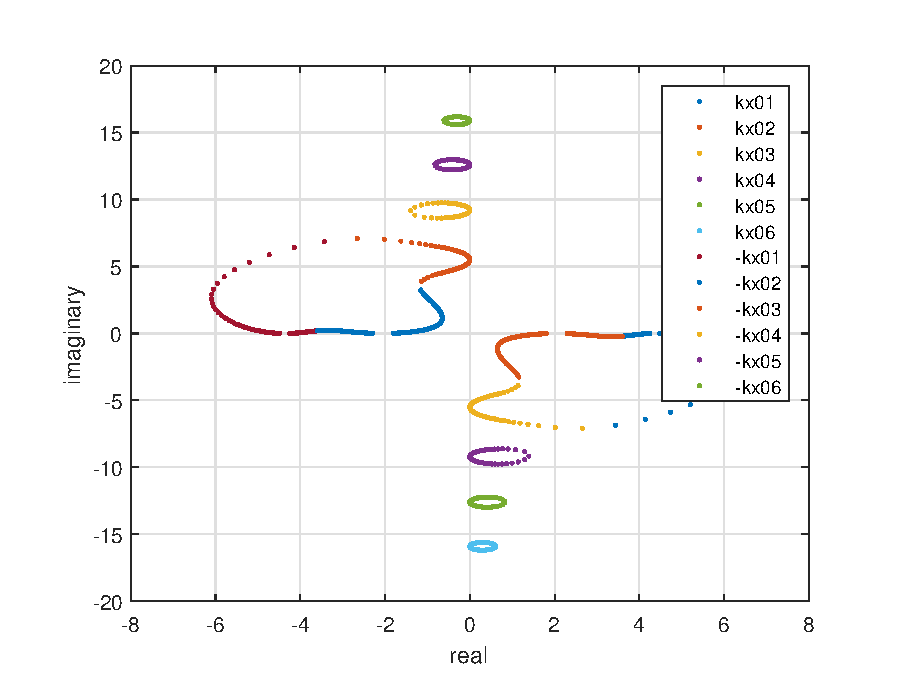
\includegraphics[width=1.13\linewidth]{kx01_05}
     \caption{$real(Z)=0.5$ and $im(Z)=-\infty \ to +\infty$}
    \end{subfigure}%
    \begin{subfigure}{.5\textwidth}\centering
     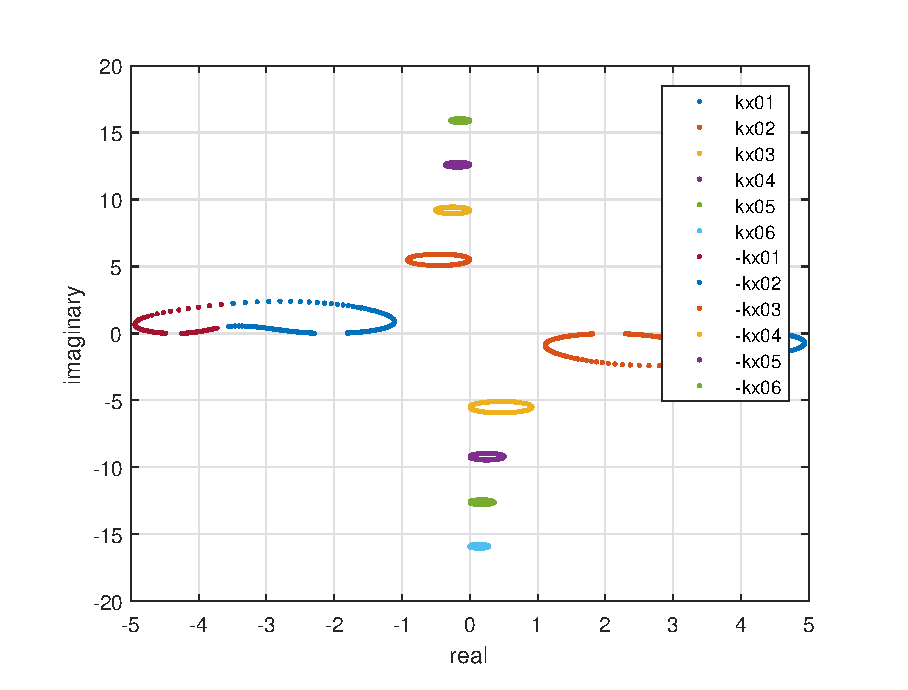
\includegraphics[width=1.13\linewidth]{kx01_10}
     \caption{$real(Z)=1$ and $im(Z)=-\infty \ to +\infty$}
    \end{subfigure}\\
    \begin{subfigure}{.5\textwidth}\centering
     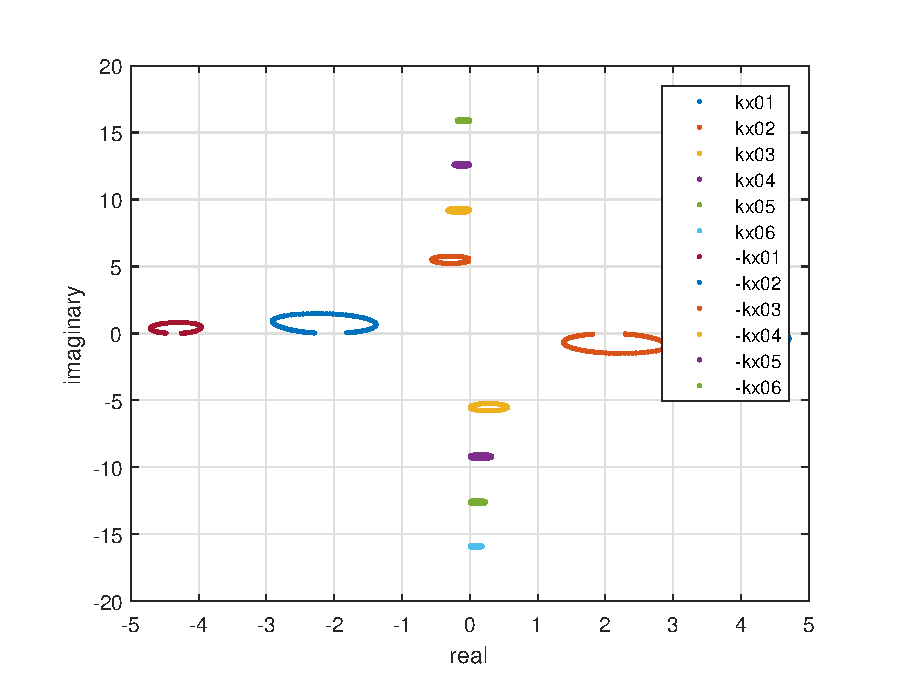
\includegraphics[width=1.13\linewidth]{kx01_15}
     \caption{$real(Z)=1.5$ and $im(Z)=-\infty \ to +\infty$}
    \end{subfigure}%
    \begin{subfigure}{.5\textwidth}\centering
     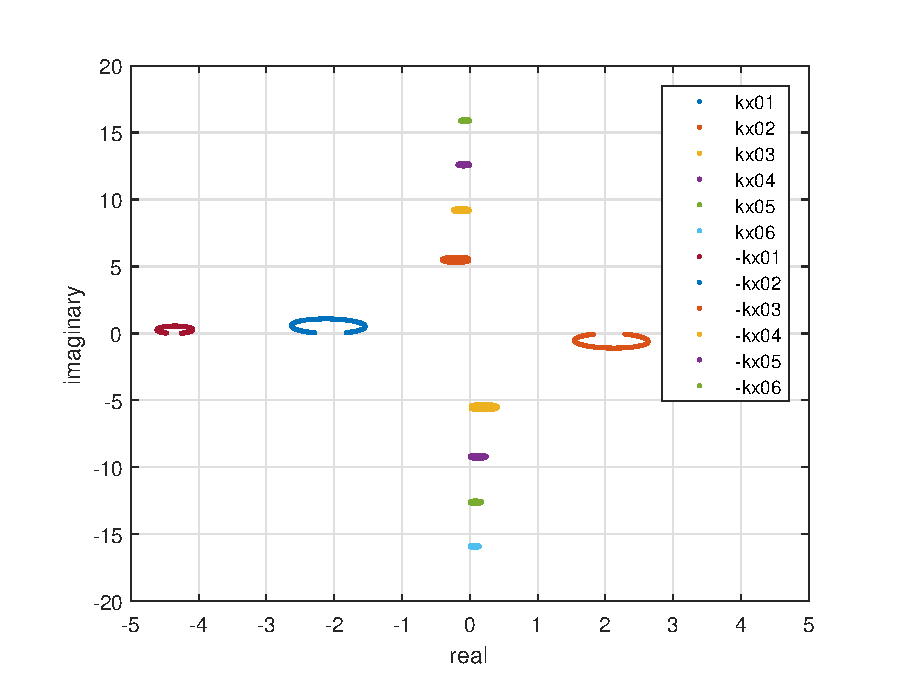
\includegraphics[width=1.13\linewidth]{kx01_20}
     \caption{$real(Z)=2$ and $im(Z)=-\infty \ to +\infty$}
    \end{subfigure}
    \caption{Axial wave numbers for $m=0,kR=4.353$ \cite{Kabral_thesis}}
\end{figure}
\noindent Cremer was the first to show the existence of a optimum radial wave number leading to the maximal axial decay rate of the least attenuate mode. This optimum condition correspond of the merging of two sequential order modes. For this specific condition the two modes collapse \cite{An_Introduction_to_Acoustics}.
\begin{figure}[H] \centering
    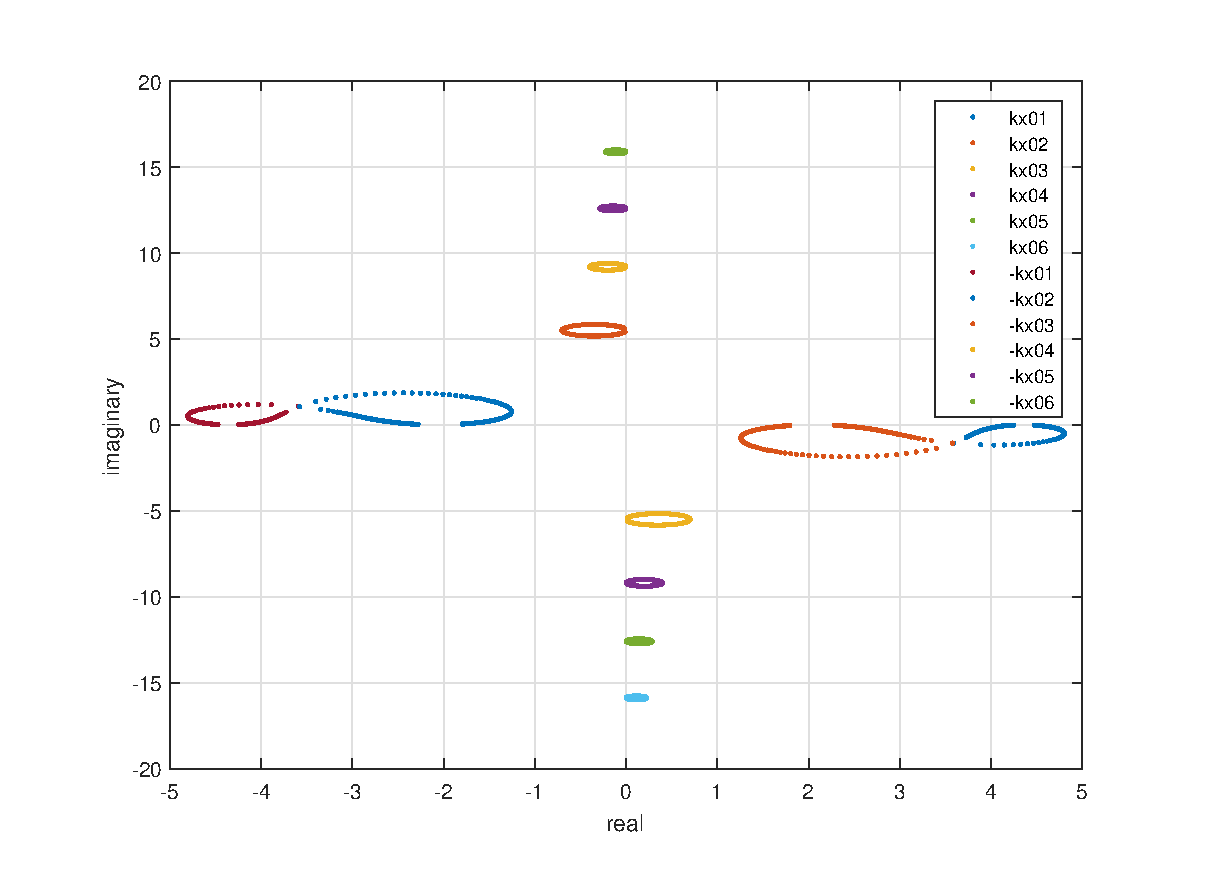
\includegraphics[scale=0.7]{kx01_Opt}
    \caption{Axial wave number in the complex plan for Im(Z) varying from -$\infty$ to +$\infty$\ and for Re(Z)=1.4165. For Im(Z)=-0.608 the first two modes coalesce $k_{01}=k_{02}=4.3-0.88i$ \cite{An_Introduction_to_Acoustics}}
\end{figure}
Cremer and Tester showed that this optimum wave number is given then the derived eigenvalue equation vanishes.
%------------------------------------------------------------------------------------------------------------
%------------------------------------------------------------------------------------------------------------
\subsubsection{Optimization of a circular liner}

The lest attenuate mode was found in an experimental setup and is the $(1,0)$. To simplify the notation $k_r=k_{r,(1,0)}$ is used. The assumption of high frequency is made \cite{Kabral_thesis}: 
\begin{equation}
    k_x\approx\frac{k}{1\pm M_x}
\end{equation}
The eigenvalue for the $(1,0)$ mode is:
\begin{equation}
   \frac{ikR}{Z}=(1\pm M_x)^2 \frac{k_r r J_1^' (k_r r)}{J_1(k_r r)}
\end{equation}
The optimum radial wave number is:
\begin{equation}
    \frac{d}{dk_r r}\Bigg[(1\pm M_x)^2 \frac{k_r r J_1^' (k_r r)}{J_1(k_r r)}\Bigg]=0
\end{equation}
The equation is solved with the Matlab function "vpsolve". The optimum impedance determined is: 
\begin{equation}
    Z=   0.8918 - 0.3068i
\end{equation}
\begin{figure}[H] \centering
    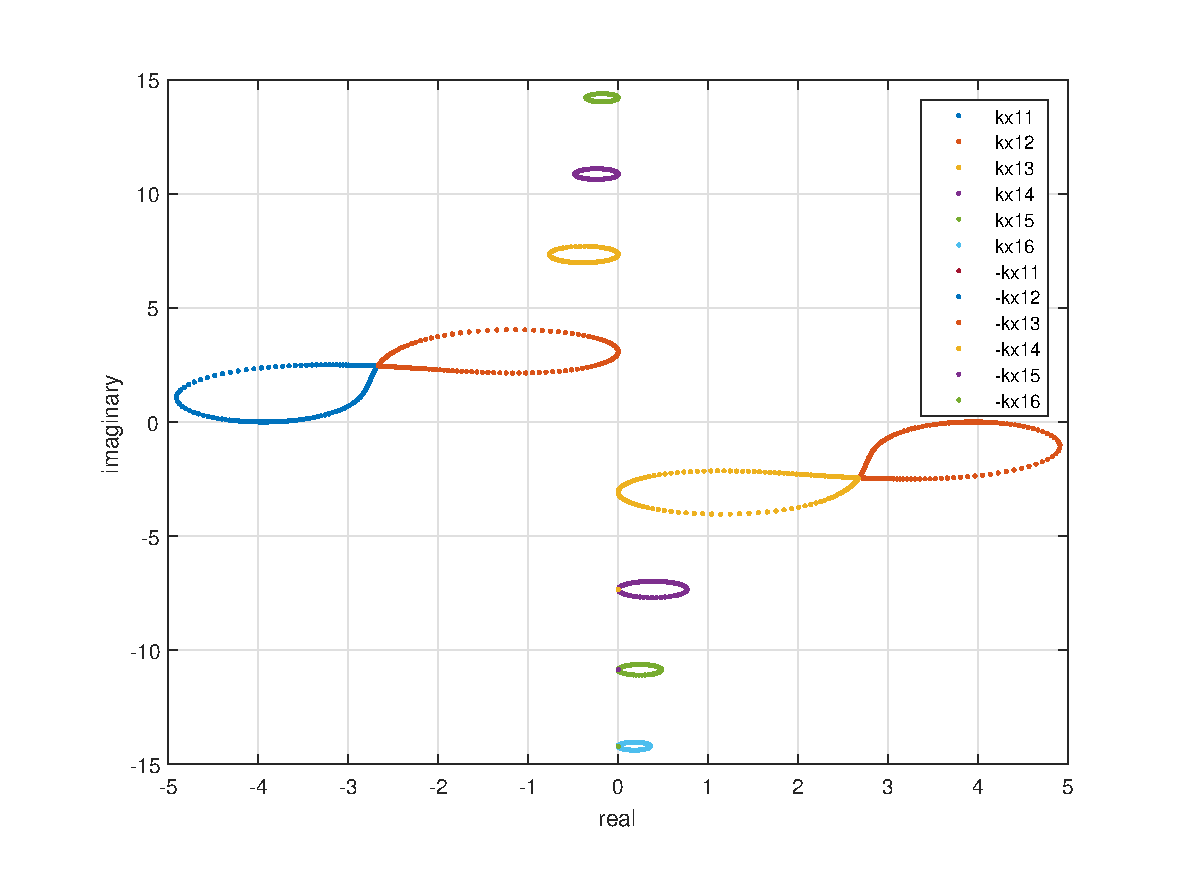
\includegraphics[scale=0.7]{kx11_OptCirc}
    \caption{Axial wave number in the complex plan for Im(Z) varying from -$\infty$ to +$\infty$\ and for Re(Z)=0.892. For Im(Z)=-0.307i the first two modes coalesce $k_{01}=k_{02}=4.4663 + 1.467i$ \cite{An_Introduction_to_Acoustics}}
\end{figure}
%------------------------------------------------------------------------------------------------------------
%------------------------------------------------------------------------------------------------------------
\subsubsection{Optimization of an annular liner}
The optimization of an annular liner is more difficult and is rarely done by an analytically method. On the contrary with the circular duct, the eigenvalue solutions are not simple. The second problem is that the least attenuate mode is rarely the plane wave mode. For our case, the least attenuate mode was the $(8,0)$ and was determined by an experimental work. We tried to implement the Cremer impedance to reduce this mode.
The general solution of the pressure field for annular ducts is:
\begin{equation}
    p_{(m,n)}=\Big[A_{mn}J_m(k_{r,(m,n)}r)+B_{mn}Y_m(k_{r,(m,n)}r)\Big]\cos (m\theta) e^{i(\omega t-k_{x,(m,n)}x)}
\end{equation}
Where $J$ the Bessel function of the first type and order $m$ and $Y$ the Bessel function of the second type and order $m$.\\
From the general pressure solution and the Myers boundary conditions Eq.\eqref{eq:Myers}:
\begin{equation}
    ik\beta_1\Big[1-(\frac{k_{x,(m,n)}}{k})M\Big]^2=k_{r,(m,n)}\Bigg[\frac{A_{mn}J_m^'(k_{r,(m,n)}b)+B_{mn}Y_m^'(k_{r,(m,n)}b)}{A_{mn}J_m(k_{r,(m,n)}b)+B_{mn}Y_m(k_{r,(m,n)}b)}\Bigg]
\end{equation}
\begin{equation}
    ik\beta_0\Big[1-(\frac{k_{x,(m,n)}}{k})M\Big]^2=k_{r,(m,n)}\Bigg[\frac{A_{mn}J_m^'(k_{r,(m,n)}a)+B_{mn}Y_m^'(k_{r,(m,n)}a)}{A_{mn}J_m(k_{r,(m,n)}a)+B_{mn}Y_m(k_{r,(m,n)}a)}\Bigg]
\end{equation}
With $\beta$ the admittance of the inner and external wall (radius $b$ and $a$). For our application we choose to lined the external wall $\beta_1=0$ and the flow is zero $M=0$.\\
The eigenvalue equation is following:
\begin{equation}\label{CremerAnnular}
    ika\beta_0=-k_{r,(m,n)}a\Bigg(\frac{J_m^'(k_{r,(m,n)}a)Y_m^'(k_{r,(m,n)}b)-J_m^'(k_{r,(m,n)}b)Y_m^'(k_{r,(m,n)}a)}{J_m(k_{r,(m,n)}a)Y_m^'(k_{r,(m,n)}b)-J_m^'(k_{r,(m,n)}b)Y_m(k_{r,(m,n)}a)}\Bigg)
\end{equation}
We solve $\frac{d}{d(k_r)}\Big(Eq.\eqref{CremerAnnular}\Big)=0$ to find the optimum $k_{r,(m,n)}$. Then Eq.\eqref{CremerAnnular} is evaluated for this optimum wave number and gives the impedance.\\
The optimum impedance is: 
\begin{equation}
    Z=0.4537 + 0.0148i
\end{equation}\\
The eigenvalue equation has $n$ solutions. To attenuate the modes $(m,n)$, the first $m$ non zero solution has to be taken. The resolution is more detailed in \nameref{sec:AppendixB}.
\clearpage
 
\section{Measurement and post-treatment}
This part describes the experimental work from the setup to the calculation of the acoustic impedance. The post-treatment is also present in this part, but the theory is already describes in \ref{sec:section2} \nameref{sec:section2}.
%------------------------------------------------------------------------------------------------------------
%------------------------------------------------------------------------------------------------------------
\subsection{Experimental work}
%------------------------------------------------------------------------------------------------------------
%------------------------------------------------------------------------------------------------------------
\subsubsection{KTH facilities}
The Marcus Wallenberg Laboratory for Sound and Vibration has a flow test rig. The sketch of the facilities:
\begin{figure}[H] \centering
    \includegraphics[scale=0.6]{MWL_flow_acoustic_test_rig}
    \caption{MWL flow acoustic test rig}
\end{figure}
The laboratory is equipped with a huge fan. For our experiments, this fan was link to the anechoic room. The pressure increases and a flow was created in a rectangular rig. The anechoic room reduces the sound produced by the fan into the rig. This fan was controlled by a computer. During my master thesis, we had to fix the cooling system to be able to run the fan at 100\% of its capacity. 
\begin{figure}[H] \centering
    \includegraphics[scale=0.05]{ExpSetup3}
    \caption{Picture of the fan software}
\end{figure}\clearpage
%------------------------------------------------------------------------------------------------------------
%------------------------------------------------------------------------------------------------------------
\subsubsection{The rig setup}
The setup is divided in three parts: 
\begin{itemize}
    \item Upstream numbered 1
    \item Lined section numbered 2
    \item Downstream numbered 3
\end{itemize}
\begin{figure}[H] \centering
    \includegraphics[scale=0.4]{Sketch_KTH_rig}
    \caption{Sketch of liner test setup at KTH}
\end{figure}
2 loudspeakers and 16 microphones were used:
\begin{itemize}
    \item 6 microphones to do the wave decomposition (3 at each upstream and downstream sides). Note than that 4 microphones were supposed to be used at the beginning.
    \item 10 microphones in the lined sections to measure the pressure field.
\end{itemize}
The termination of the rig is composed by a muffler. The reflection was very low but not equal to zero at the end of the rig.
\begin{figure}[H] \centering
    \includegraphics[scale=0.1]{ExpSetup1}
    \caption{Picture of the Rig and the anechoic termination}
\end{figure}
\begin{figure}[H] \centering
    \includegraphics[scale=0.1]{ExpSetup2}
    \caption{Picture of the 16 microphones and the downstream loudspeaker}
\end{figure}
\noindent The liner is fixed flush with the wall. Any leakage can change the acoustic field.
\begin{figure}[H] \centering
    \includegraphics[scale=0.08]{ExpSetup5}
    \caption{Picture of the acoustic liner fixed in the rig}
\end{figure}
\noindent The velocity of the flow has to be measured. The \nameref{sec:AppendixC} describes how to get the mean flow in the duct with the Pitot tube.
\begin{figure}[H] \centering
    \includegraphics[scale=0.05]{ExpSetup4}
    \caption{Picture of the Pitot tube}
\end{figure}
%------------------------------------------------------------------------------------------------------------
%------------------------------------------------------------------------------------------------------------
\subsubsection{Acquisition chain}
\begin{figure}[H] \centering
    \begin{subfigure}{.5\textwidth}\centering
     \includegraphics[width=.8\linewidth]{Acquisition1}
     \caption{Picture computer and nexuses}
    \end{subfigure}%
    \begin{subfigure}{.5\textwidth}\centering
     \includegraphics[width=.8\linewidth]{Acquisition2}  
      \caption{Picture of the  calibration tube}
    \end{subfigure}
    \caption{Pictures of experimental devices}
\end{figure}
\noindent A HP-VXI system creates an sinus excitation signal. This sinal is amplified by a classic amplifier and the loudspeaker transforms the signal into an acoustic sinus wave. The Brüel and Kjaer microphones provide an electric signal which is treat by a Nexus device. To get the true pressure value, the sensitivity and the gain of the nexus have to be saved. The HP-VXI system does also the acquisition. A Matlab program saves the temporal data into a file.\\
This code provides by Luck \cite{Luck_thesis} has also other options to improve the quality of the measure:
\begin{itemize}
    \item The excitation is calibrated before the measure to respect a positive plane wave $p^+$ equal to $1Pa$. This calibration should avoid any non-linear pressure effect (this option is more important for high excitation level)
    \item The time of the acquisition depends of the variance of the measured signals. The accuracy of the data increases with the measured time. But the temperature into the rig increases slowly during the measurement. The measure has to relatively fast to avoid any temperature effect.
    \item By the same idea, the frequencies studied are randomized. The effect of the temperature variation are distributed, and any temperature trend appears.
\end{itemize}
To get a more accuracy measure, the microphones are calibrated before. A stationary wave is created in a tube. The axial position of the microphones are strictly the same as are the measured pressures. The transfer functions are calculated, the reference is the first microphone.
%------------------------------------------------------------------------------------------------------------
\subsubsection{Frequency domain and scattering matrix}
The measures are time dependant: 
\begin{figure}[H] \centering
    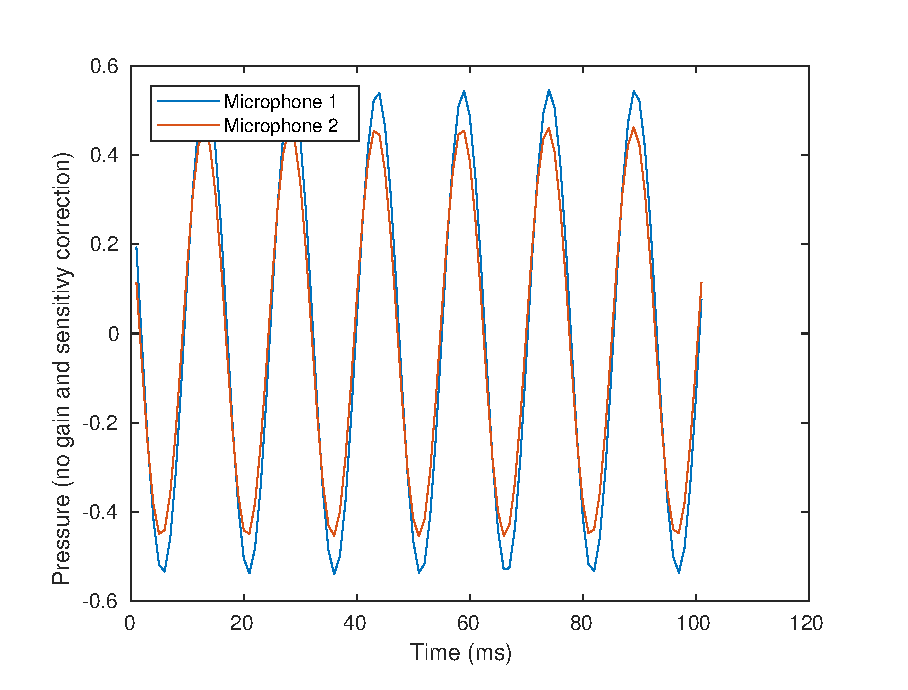
\includegraphics[scale=0.7]{PTimeNoLiner}
    \caption{Time dependant signal}
\end{figure}
The Hilbert transform is used to get the estimated transfer function:
\begin{figure}[H] \centering
    \includegraphics[scale=0.7]{PHilbertNoLiner}
    \caption{Estimated transfer function time dependant before windows filtering}
\end{figure}
A windows is determined which contained a whole number of sinus. The signal is filtered to get the true transfer function:
\begin{figure}[H] \centering
    \includegraphics[scale=0.7]{PHilbertFiltreNoLiner}
    \caption{True transfer function time dependant after windows filtering}
\end{figure}
With the source reference, all the complex pressures are determined.
%------------------------------------------------------------------------------------------------------------
%------------------------------------------------------------------------------------------------------------
\subsection{Reference: hard wall case}
3 mach flows are studied: $M=0, M=0,08\ \text{and}\ M=0.16$. The frequency is between 700Hz and 1200Hz.\\
It's very difficult to get accurate measures in a rig. The mean flow adds lot of in-stationary noise. In a way to gain confidence in the results, a measure of the hard wall duct are performed. The problem is reduce to an infinite hard duct. Only a plane wave propagates because the higher modes are over the cut-off frequency. In this simple case the two transmission coefficients should be 1 and the reflecxion coefficients equal to zero.\\
The scattering matrix measured:
\begin{figure}[H] \centering
    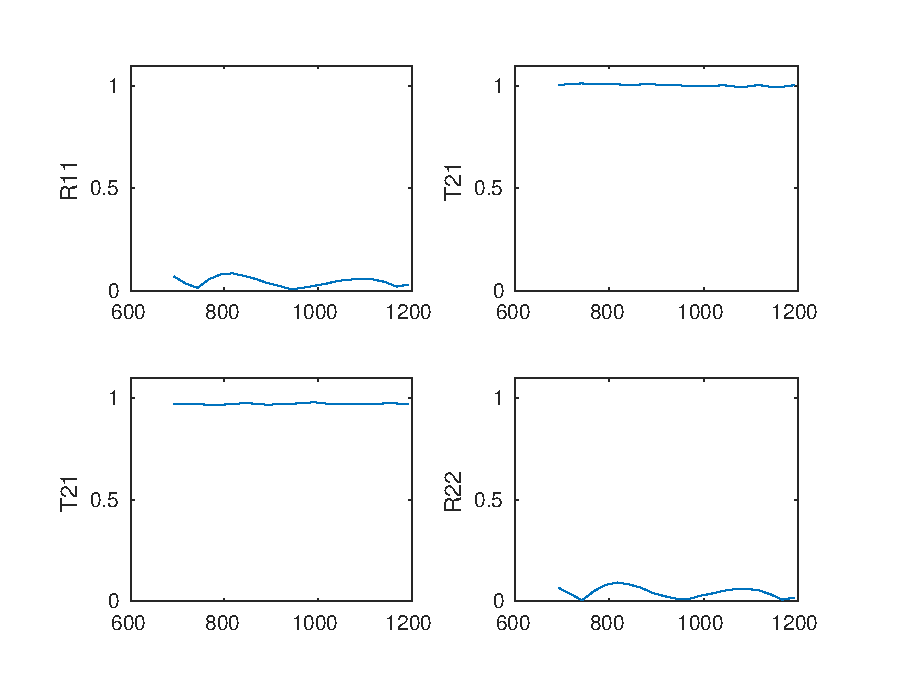
\includegraphics[scale=0.7]{ScatNoLin}
    \caption{Scattering matrix: Hard wall and no flow }
\end{figure}
\noindent The transmission coefficients are very close to 1. The reflection is a little bit higher than expected. With flow, the scattering matrix stay very accurate:
\begin{figure}[H] \centering
    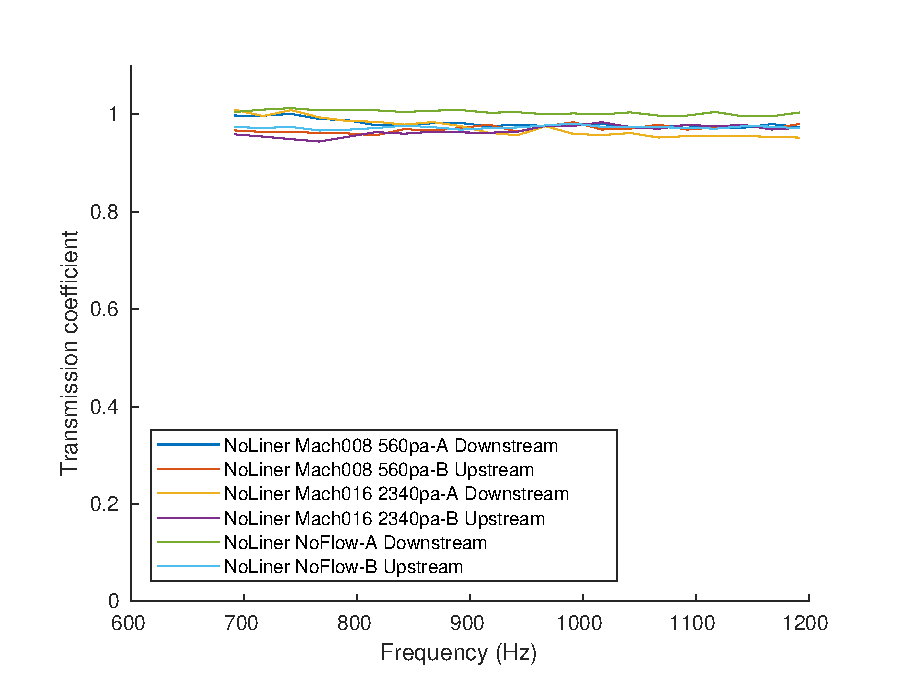
\includegraphics[scale=0.7]{TNoLinAll}
    \caption{Transmission coefficients (T21 correspond to upstream and  T12 correspond to downstream excitation): Hard wall; M=0, M=0.08, M=0.16 }
\end{figure}
%------------------------------------------------------------------------------------------------------------
%------------------------------------------------------------------------------------------------------------
%------------------------------------------------------------------------------------------------------------
%------------------------------------------------------------------------------------------------------------
\subsection{Acoustic liner}
%------------------------------------------------------------------------------------------------------------
%------------------------------------------------------------------------------------------------------------
\subsubsection{Scattering matrix and transmission loss}
\begin{figure}[H] \centering
    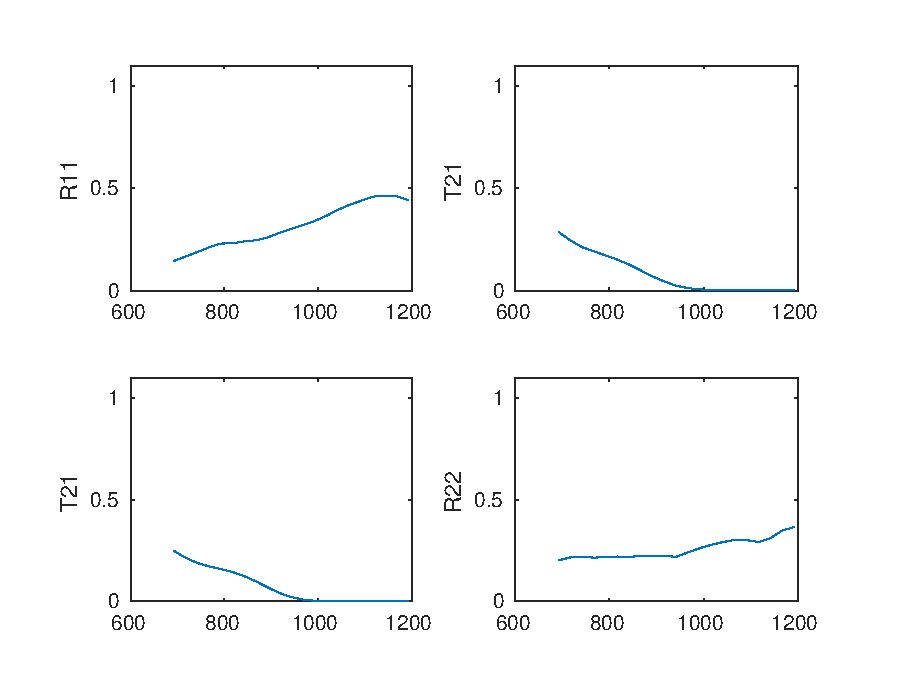
\includegraphics[scale=0.7]{ScatLinNoFlow}
    \caption{Scattering matrix: Liner and no flow}
\end{figure}
The reflection is lower than 0.5. Some energy is reflected towards the source.\\
A liner has to reduce the acoustic energy transmit to the output.
The transmission loss is directly given by the transmission coefficient:
\begin{equation}
    TL=20\text{log}(1/T)
\end{equation}
Thus, the studied parameter is the transmission coefficient. As a reminder, upstream transmission coefficient is called $T12$ and the downstream $T21$. For every case this coefficient is closed to zero, almost all the acoustic energy is absorbed or reflected.\\
These coefficients are equal for no flow. But more the velocity is high more the upstream transmission becomes higher than the downstream transmission. This effect is due to the non uniform shape flow. At the wall the acoustic wave sees an opposite velocity gradient for the upstream or downstream propagation. This effect is not taken account in the Myers boundary conditions which consider uniform flow. This difference is showed: 
\begin{figure}[H] \centering
    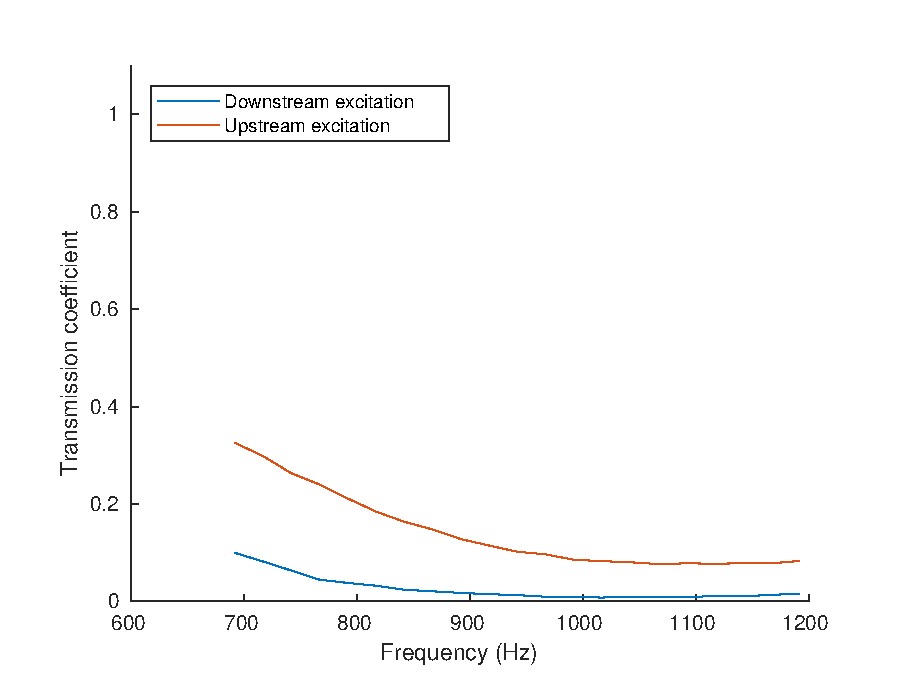
\includegraphics[scale=0.7]{TLinM016}
    \caption{Transmission coefficients: Liner 1 and M=016}
\end{figure}
Two different effects of the flow are highlighted:
\begin{itemize}
    \item Upstream excitation: the transmission increases with the mach number at low frequency
    \item downstream excitation: the efficiency of the liner increases at low frequency.
\end{itemize}
\begin{figure}[H] \centering
    \begin{subfigure}{.5\textwidth}\centering
     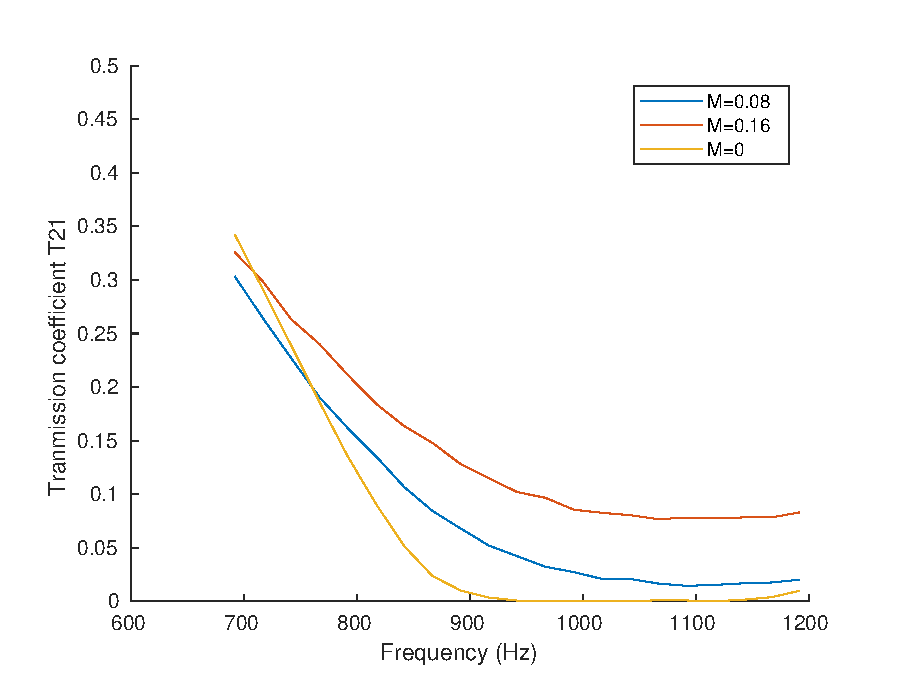
\includegraphics[width=1\linewidth]{T21Lin1}
    \caption{T21}
    \end{subfigure}%
    \begin{subfigure}{.5\textwidth}\centering
     \includegraphics[width=1\linewidth]{T12Lin1}
    \caption{T12}
    \end{subfigure}
    \caption{Transmission coefficients: Liner 1 and M=0, M=0.08, M=0.16}
\end{figure}
Liners should have the same dimensions and the same acoustic properties. However, no-negligible difference between these liners are highlighted:
\begin{figure}[H] \centering
    \includegraphics[scale=0.7]{T12M016}
    \caption{Transmission coefficients: liner 1, liner 2, liner 3 for M=0.16 }
\end{figure}
The first results show the expected trends. The setup shows a good repeatability. Indeed two measures with the same liner were done (Two different fixations) and they are very closed.\\
The difference between the liners stays unexplained.
\subsubsection{Acoustic impedance}
A second step of post-treatment is to get the acoustic impedance.

%------------------------------------------------------------------------------------------------------------
%------------------------------------------------------------------------------------------------------------
\clearpage 
%\section{Results and discussion}
%------------------------------------------------------------------------------------------------------------
%------------------------------------------------------------------------------------------------------------
\subsection{Results compare to the theory}
%------------------------------------------------------------------------------------------------------------
%------------------------------------------------------------------------------------------------------------
%------------------------------------------------------------------------------------------------------------
%------------------------------------------------------------------------------------------------------------
\subsection{Difference between the liner}
%------------------------------------------------------------------------------------------------------------
%------------------------------------------------------------------------------------------------------------
%------------------------------------------------------------------------------------------------------------
%------------------------------------------------------------------------------------------------------------
\clearpage 
\setlength{\parskip}{5pt}
\setlength\parindent{20pt}
\section{Conclusion}
\setlength{\parindent}{20pt}
 \indent Measures in a flow rig ask theoretic knowledge. The specificity of the duct acoustic is the possibility to work with the modes because of the low amount of them. 
 
 Resolve the convective Helmholtz equation allows to describes these modes and their shapes. In the axial direction a positive and a negative wave can propagate, the modes have different shapes in the section. For the rectangular duct, the different waves numbers are link but the modes are independent in each direction. While for the annular case the circumferential and the radial modes are linked by a Bessel function.
The optimization of an acoustic liner is not easy for two main reasons: 
\begin{itemize}
    \item The dimension of the duct are very high compare to the dimensions of the liner cavities. The problem asks too many resources for numerical methods. The acoustic impedance has to be used to simplify the problem.
    \item The acoustic theory for lined wall in a circular duct is though. The optimum Tester and Cremer impedance is well determined to reduce the plane wave mode in a circular duct. In this master thesis, we tried to generalize for a higher mode and for the annular case 
\end{itemize}
\indent To get the acoustic properties some works have to be done into the time data. This post-treatment is based on models and adds some uncertainties into the final values.

Last but not least the measurement with flow must be done carefully. The noise created by the flow is important.

The first results show a high transmission loss. However the disparity of the 3 liners seems to be high. The future determination of the impedance will confirm if something is wrong. There were some manufactured defaults in the Chinese liners what can explain this disparity.
\clearpage

 

\bibliographystyle{unsrtnat}
%\bibliographystyle{plain}
\bibliography{references}
\clearpage
\pagestyle{empty}
\setlength{\parskip}{0pt}
\setlength\parindent{0pt}
\section{Appendix}\label{sec:Annexes}
%------------------------------------------------------------------------------------------------------------
%------------------------------------------------------------------------------------------------------------
%------------------------------------------------------------------------------------------------------------
%------------------------------------------------------------------------------------------------------------
\subsection*{Appendix A: Modes for rectangular duct}\label{sec:EigenvalueRect}
The duct geometry is:
\begin{figure}[H] \centering
    \includegraphics[scale=0.3]{Zhourectduct}
    \caption{Rectangular duct lined for y=-a}
\end{figure}
The Convective Helmholtz equation in the Cartesian coordinates:
\begin{equation}
    \Delta p +\Big[(w-ku_0)^2-k^2c_0^2\Big]p=0
\end{equation}
A resolution by separation of variables gives this decomposition:
\begin{equation}
    p(x,y,z,\omega)=\sum_{l=0}^\infty p_l^+ \Psi_{(m,n)}(x,y,z)+p_l^- \Psi_{(m,n)}(x,y,z)
\end{equation}
With:
\begin{equation}
    \Psi_{(m,n)}(x,y,z)=(A_me^{ik_{y,(m,n)}}+B_me^{-ik_{y,(m,n)}})(A_ne^{ik_{z,(m,n)}}+B_ne^{-ik_{z,(m,n)}})e^{-ik_{x,(m,n)}(M,\omega)x}
\end{equation}
%------------------------------------------------------------------------------------------------------------
%------------------------------------------------------------------------------------------------------------
\subsubsection*{Hard duct}\label{sec:EigenvalueHard}
Starting with the general form:
\begin{equation}
        \Psi(x,y,z)=(Ae^{ik_{y}y}+Be^{-ik_{y,l}y})(Ce^{ik_{z}z}+Dne^{-ik_{z}z})e^{-ik_{x}(M,\omega)x}
\end{equation}
The boundary conditions in the z direction are the hard wall conditions, the velocity is zero:  
\begin{equation}
    \frac{\partial\Psi}{\partial z} \Bigg|_{z=+a}=0
\end{equation}
Give the system:
\begin{equation}\label{eq:1}
    \left\{
    \begin{array}{ll}
    Ce^{-ik_za}-De^{ik_za}=0\\
        \\
    Ce^{ik_za}-De^{-ik_za}=0   
    \end{array}
    \right.
\end{equation}
In the matrix form: 
\begin{gather}
    \begin{bmatrix}
      e^{-ik_za} & -e^{ik_za} \\
      e^{ik_za} & -e^{-ik_za}
    \end{bmatrix}
    \begin{pmatrix}
       C\\
       D
    \end{pmatrix}
    =
    \begin{pmatrix}
      0\\
      0
    \end{pmatrix}
\end{gather}
The eigenvalue equation:
\begin{equation}
    -e^{-i2k_za}+e^{i2k_za}=0 \iff \sin(2ka)=0
\end{equation}
The wave number of order $n$:
\begin{equation}
    k_{z,n}=\frac{n\pi}{2a} \ ; \ n\in N
\end{equation}
Compute in the system Eq.\eqref{eq:1}
\begin{equation}
    \left\{
    \begin{array}{ll}
    C_ne^{-i\frac{n\pi}{2}}-D_ne^{i\frac{n\pi}{2}}=0\\
        \\
    C_ne^{i\frac{n\pi}{2}}-D_ne^{-i\frac{n\pi}{2}}=0   
    \end{array}
    \right.
\end{equation}
Thus:
\begin{equation}
    C_n(-i)^{n}-D_n(i)^{n}=0
\end{equation}
Two cases $n=2p$ or $n=2p+1$
\begin{equation}
    C_n=D_n \ \text{for} \ n=2p \ \text{and} \ C_n=-D_n\ \text{for} \ n=2p+1 
\end{equation}
Two solution for the shapes modes:
\begin{equation}
    \Psi_{n}(z)=2\cos(\frac{n\pi}{2a}z) \ \text{for} \ n=2p \ \text{and} \ \Psi_{n}(z)=2i\sin(\frac{n\pi}{2a}z)\ \text{for} \ n=2p+1 
\end{equation}
Finally for two opposite hard walls the shapes modes are: 
\begin{equation}
    \left\{
    \begin{array}{ll}
    \Psi_{n}(z)=2\cos(\frac{n\pi}{2a}z)\ \text{for} \ n=2p \\
        \\
    \Psi_{n}(z)=2i\sin(\frac{n\pi}{2a}z) \ \text{for} \ n=2p+1
    \end{array}
    \right.
\end{equation}
Note that only the modes below the cut-off frequency propagate. The higher mode are quickly attenuated. 
%------------------------------------------------------------------------------------------------------------
%------------------------------------------------------------------------------------------------------------
\subsubsection*{Lined walls}\label{sec:EigenvalueLined}
Starting with the general form:
\begin{equation}
        \Psi(x,y,z)=(Ae^{ik_{y}y}+Be^{-ik_{y,l}y})(Ce^{ik_{z}z}+Dne^{-ik_{z}z})e^{-ik_{x}(M,\omega)x}
\end{equation}
The boundary conditions in the y direction one lined wall and a hard wall, the velocity is respectively 0 and given by the Myers condition:
\begin{equation}
    \frac{\partial\Psi}{\partial y} \Big|_{y=+a}=0
\end{equation}
\begin{equation}
    \frac{\partial p}{\partial y}\Bigg|_{y=-a}=\frac{ik}{Z}(1-iM\frac{\partial}{\partial x})^2 p\Bigg|_{y=-a}
\end{equation}
Give the system:
\begin{equation}\label{eq:2}
    \left\{
    \begin{array}{ll}
    Ae^{ik_ya}-Be^{-ik_ya}=0\\
        \\
    Aik_ye^{-ik_ya}-Bik_ye^{ik_ya}=ikA(1-\frac{Mk_x}{k})[Ae^{-ik_ya}-Be^{ik_ya}]
    \end{array}
    \right.
\end{equation}
Using the wave dispersion equation:
\begin{equation}
   k_z^2+k_y^2=(k-Mk_x)^2 
\end{equation}
Using this relation in the Myers condition:
\begin{equation}
    \left\{
    \begin{array}{ll}
    Ae^{ik_ya}-Be^{-ik_ya}=0\\
        \\
    Ak_ye^{-ik_ya}-Bk_ye^{ik_ya}=\frac{A}{k}(k_z^2+k_y^2)^2[Ae^{-k_ya}-Be^{k_ya}]
    \end{array}
    \right.
\end{equation}\label{eq:3}
The matrix form: 
 \begin{gather}
    \begin{bmatrix}
     e^{ik_ya} & -e^{-ik_ya} \\
      \\
     k_ye^{-ik_ya}-\frac{A}{k}(k_z^2+k_y^2)^2[e^{-k_ya}] & -k_ye^{ik_ya}-\frac{A}{k}(k_z^2+k_y^2)^2[-e^{k_ya}]
    \end{bmatrix}
    \begin{pmatrix}
       A\\
       B
    \end{pmatrix}
    =
    \begin{pmatrix}
      0\\
      0
    \end{pmatrix}
 \end{gather}
The eigenvalue equation:
\begin{equation}
    -k_y(e^{i2k_ya}-e^{-i2k_ya})-(e^{2ik_ya}+e^{-2ik_ya})(\frac{A}{k}(k_z^2+k_y^2))=0
\end{equation}
The final eigenvalue equation:
\begin{equation} \label{eq:eigenlined}
    k_y\tan(2k_ya) -i(\frac{A}{k}(k_z^2+k_y^2))=0
\end{equation}
This equation has $m$ solution, called modes. Thus the wave number $k_{y,m}$ is the $m-th$ $k_r$ solution of the eigenvalue equation Eq.\eqref{eq:eigenlined}. 
The first line of the system Eq.\eqref{eq:3} gives an other condition for the amplitudes:
\begin{equation}
    A_me^{ik_{y,m}a}-B_me^{-ik_{y,m}a}=0 \iff  B_m=A_me^{i2k_{y,m}a}
\end{equation}
Finally for a lined wall opposite to a hard walls the shapes modes are: 
\begin{equation}
    \Psi_{m}(y)=e^{ik_{y,m}y}-e^{-ik_{y,m}(y-2a)}\ \text{with}\ k_{y,m} \ \text{solution of} \ Eq.\eqref{eq:eigenlined}
\end{equation}
Note than the relation:
\begin{equation}
   \frac{\frac{\partial\Psi_{l}}{\partial y}|_{y=-a}}{p|_{y=-a}}=k_y\tan(2k_ya)
\end{equation}
And compute in the Myers boundary conditions gives directly the impedance:
\begin{equation}\label{eq:Impedance}
   Z=\frac{i(k-Mk_x)^2}{k\ k_z\tan(2ak_x)}
\end{equation}
%------------------------------------------------------------------------------------------------------------
%------------------------------------------------------------------------------------------------------------
%------------------------------------------------------------------------------------------------------------
%------------------------------------------------------------------------------------------------------------
\subsection*{Appendix B: Cremer optimum resolution with matlab}\label{sec:AppendixB}
The circular resolution is very similar to the annular resolution.
The least attenuated mode is the $(m,n)$ and the radial wave number is $k_r=k_{r,(m,n)}$. A function $F(k_r)$ is defined as the derivative of the eigenvalue equation. The function "vpsole" solve $F=0$ using a starting point called "initial guess". \\
To preliminary find the "initial guess point", $1/F(k_r)$ is ploted in the complex plan: 
\begin{figure}[H] \centering
    \includegraphics[scale=0.3]{1_Fctannulaire13D}
    \caption{$1/F(k_r)$ in the complex plan}
\end{figure}
Every peak correspond to a root of $F(k_r)$ and the approximate coordinates are used in the "vpsovle" as initial guess.\\
The first $n$ solutions are represented in the graph:
\begin{figure}[H] \centering
    \includegraphics[scale=0.7]{Solutionscyl2D}
    \caption{$k_{r,(1,n)}$ solution of $F=0$ for the circular case}
\end{figure}
The $n$ non zero is the optimum radial wave number $k_{r,(m,n)}$ 
%------------------------------------------------------------------------------------------------------------
%------------------------------------------------------------------------------------------------------------
%------------------------------------------------------------------------------------------------------------
%------------------------------------------------------------------------------------------------------------
\subsection*{Appendix C: Mean flow measurement}\label{sec:AppendixC}
The Pitot tube measures the dynamic $p_t$ pressure thanks to a manometer. The atmospheric pressure is called $P_s$.
Two models exist:
\begin{itemize}
    \item Incompressible fluid
        \begin{equation}
        u = \sqrt{\frac{2(p_t-p_s)}{\rho}}         
        \end{equation}
        \item Compressible fluid
        \begin{equation}
        \frac{p_t}{p_s} = \Big(1+\frac{\gamma-1}{2}  M^2\Big)^{\frac{\gamma}{\gamma-1}}    
        \end{equation}
\end{itemize}
The two models are drawn in a graphic:
\begin{figure}[H] \centering
    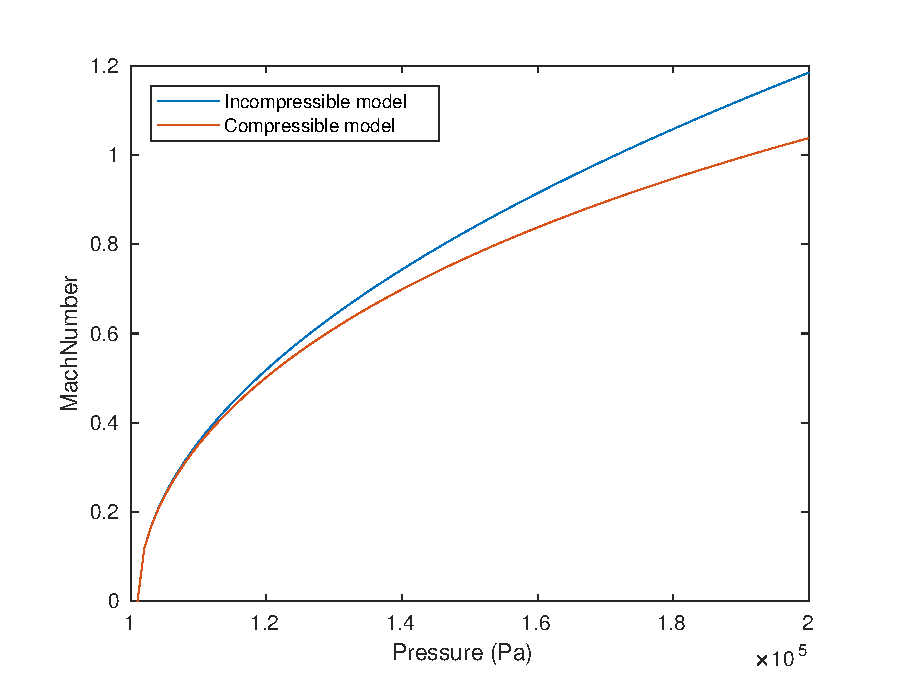
\includegraphics[scale=0.7]{MachModels}
    \caption{Two different models for Pitot tube}
\end{figure}
\noindent For mach number belove $0.2$ both models give approximately the same value.\\
However, the pressure is measured in the middle of the section and get the maximal velocity. Indeed the profil of the velocity across the section is not uniform as showed the following graphic:
\begin{figure}[H] \centering
    \includegraphics[scale=0.2]{FlowProfil}
    \caption{Flow profile across a section \cite{Zhou_thesis}}
\end{figure}
\noindent A correction coefficient between the mean mach number and the maximum mach number is applied. It was determined with a linear regression based on experimental values \cite{Zhou_thesis}.
\begin{figure}[H] \centering
    \includegraphics[scale=0.7]{LinearRegretion}
    \caption{Linear regression}
\end{figure}
The target mach numbers used in this report were 0.08 and 0.16 and are the mean mach number value. 
\end{document}